\chapter{Fuzzy Logic}

\begin{goals}
\begin{itemize}
    \item See the simplest way to make logic continuous: fuzzy truth values
    \item Understand fuzzy AND, OR, NOT
    \item Appreciate what works and what doesn't
\end{itemize}
\end{goals}

\section{Truth as a Degree}

Classical logic: $\mathrm{true} = 1$, $\mathrm{false} = 0$.

Fuzzy logic: truth values in $[0, 1]$.

\begin{intuition}
``The water is hot'' --- is this true or false? Depends on temperature. At 30°C, maybe 0.3 true. At 80°C, maybe 0.95 true. Fuzzy logic captures this gradation.
\end{intuition}

\section{Fuzzy Connectives}

How should $\land$, $\lor$, $\neg$ work on $[0, 1]$?

\textbf{Negation}:
\[
\neg x = 1 - x
\]
If $x$ is 0.7 true, then $\neg x$ is 0.3 true.

\textbf{Conjunction} (Gödel):
\[
x \land y = \min(x, y)
\]
``$A$ and $B$'' is as true as the least true conjunct.

\textbf{Disjunction} (Gödel):
\[
x \lor y = \max(x, y)
\]
``$A$ or $B$'' is as true as the most true disjunct.

\section{Example: Fuzzy Kripke Model}

\begin{definition}[Fuzzy Kripke Model]
A \emph{fuzzy Kripke model} is $(W, R, V)$ where:
\begin{itemize}
    \item $R : W \times W \to [0, 1]$ (fuzzy accessibility)
    \item $V : \Phi \to (W \to [0, 1])$ (fuzzy valuation)
\end{itemize}
\end{definition}

Satisfaction becomes a degree:
\begin{align*}
\sem{p}_w &= V(p)(w) \\
\sem{\neg\varphi}_w &= 1 - \sem{\varphi}_w \\
\sem{\varphi \land \psi}_w &= \min(\sem{\varphi}_w, \sem{\psi}_w) \\
\sem{\necessary\varphi}_w &= \min_{v \in W} \left( R(w,v) \Rightarrow \sem{\varphi}_v \right)
\end{align*}

where $a \Rightarrow b = \min(1, 1 - a + b)$ (Łukasiewicz implication) or other choices.

\section{Problems with Min/Max}

\begin{warning}
Min/max have zero gradients almost everywhere!

If $x = 0.3$ and $y = 0.7$, then $\min(x, y) = x$. The gradient w.r.t. $y$ is zero. Optimization gets stuck.
\end{warning}

\begin{center}
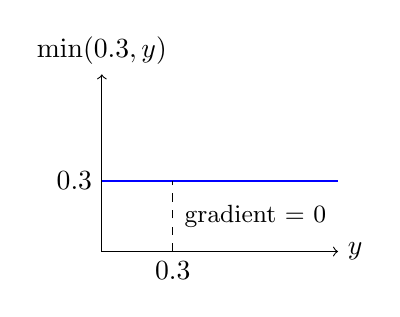
\begin{tikzpicture}[scale=1.5]
\draw[->] (0,0) -- (2,0) node[right] {$y$};
\draw[->] (0,0) -- (0,1.5) node[above] {$\min(0.3, y)$};
\draw[thick, blue] (0, 0.6) -- (0.6, 0.6);
\draw[thick, blue] (0.6, 0.6) -- (2, 0.6);
\draw[dashed] (0.6, 0) -- (0.6, 0.6);
\node[below] at (0.6, 0) {$0.3$};
\node[left] at (0, 0.6) {$0.3$};
\node at (1.3, 0.3) {\small gradient = 0};
\end{tikzpicture}
\end{center}

\section{Alternative: Product Logic}

Instead of min/max, use multiplication:
\begin{align*}
x \land y &= x \cdot y \\
x \lor y &= x + y - x \cdot y
\end{align*}

Now gradients are non-zero:
\[
\frac{\partial (x \cdot y)}{\partial y} = x \neq 0
\]

But this changes the algebraic properties...

\section{The Pattern}

We have two ``fuzzy logics'':

\begin{center}
\begin{tabular}{lll}
& \textbf{Gödel} & \textbf{Product} \\
\hline
AND & $\min$ & $\times$ \\
OR & $\max$ & $+$ (clamped) \\
\end{tabular}
\end{center}

They're both trying to do the same thing: extend Boolean logic to $[0,1]$.

Is there a general framework that includes both?
